% I. Anexo técnico: hardware (Guía apdo. 3.I)
% Los anexos NO cuentan para las 25-50 páginas. Aquí va el detalle reproducible.
% Fuentes de verdad: README.md (pinout), docs/HARDWARE_NOTES.md
\chapter{Anexo técnico: hardware y montaje}
\label{anexo:hardware}

\section{Esquema de conexiones}

El cuadro~\ref{table:pinout} recoge el conexionado completo del nodo.

\begin{table}[ht!]
\caption{Conexionado de los sensores al microcontrolador ESP32.}
\label{table:pinout}
\centering
\begin{tabular}{|p{3cm}|p{2.5cm}|p{2cm}|p{5cm}|}
\hline
\textbf{Componente} & \textbf{Pin sensor} & \textbf{Pin ESP32} & \textbf{Observaciones} \\
\hline
Todos & VCC / VDD & 3V3 & Alimentación común \\
\hline
Todos & GND & GND & Tierra común \\
\hline
MPU-6050 & SDA & GPIO 1 & Bus I\textsuperscript{2}C a \mbox{200 kHz} \\
\hline
MPU-6050 & SCL & GPIO 2 & Bus I\textsuperscript{2}C a \mbox{200 kHz} \\
\hline
DS18B20 & DATA & GPIO 14 & Bus 1-Wire; resistencia de polarización de
\mbox{5 k$\Omega$} hacia 3V3 \\
\hline
INMP441 & WS & GPIO 12 & Selección de canal (I2S) \\
\hline
INMP441 & SD & GPIO 13 & Datos de audio (I2S) \\
\hline
INMP441 & SCK & GPIO 17 & Reloj de bit (I2S) \\
\hline
INMP441 & L/R & GND & A tierra para seleccionar el canal izquierdo \\
\hline
\end{tabular}
\end{table}

La placa empleada es una DFRobot FireBeetle~2 ESP32-S3, cuyo mapa de pines no coincide con
el del ESP32 clásico. Los pines GPIO~21 y GPIO~22 habituales para el bus
I\textsuperscript{2}C no son utilizables: el GPIO~22 no existe en esta variante y el GPIO~21
corresponde al diodo emisor integrado en la placa. Los pines del bus se declaran de forma
explícita en el firmware, en lugar de heredarse del fichero de variante de la placa, para
que una actualización del entorno de compilación no los reasigne de forma silenciosa. Los
pines GPIO~33 a GPIO~37 están reservados por la memoria PSRAM octal de esta placa y no deben
cablearse.

\section{Descripción del banco de pruebas}

La figura~\ref{fig:banco-conjunto} muestra el conjunto del banco: el activo de refrigeración,
el nodo de captura situado en su base y el concentrador Raspberry~Pi, este último con cable
de red para gestión mientras su interfaz inalámbrica opera como punto de acceso.

\begin{figure}[ht!]
\centering
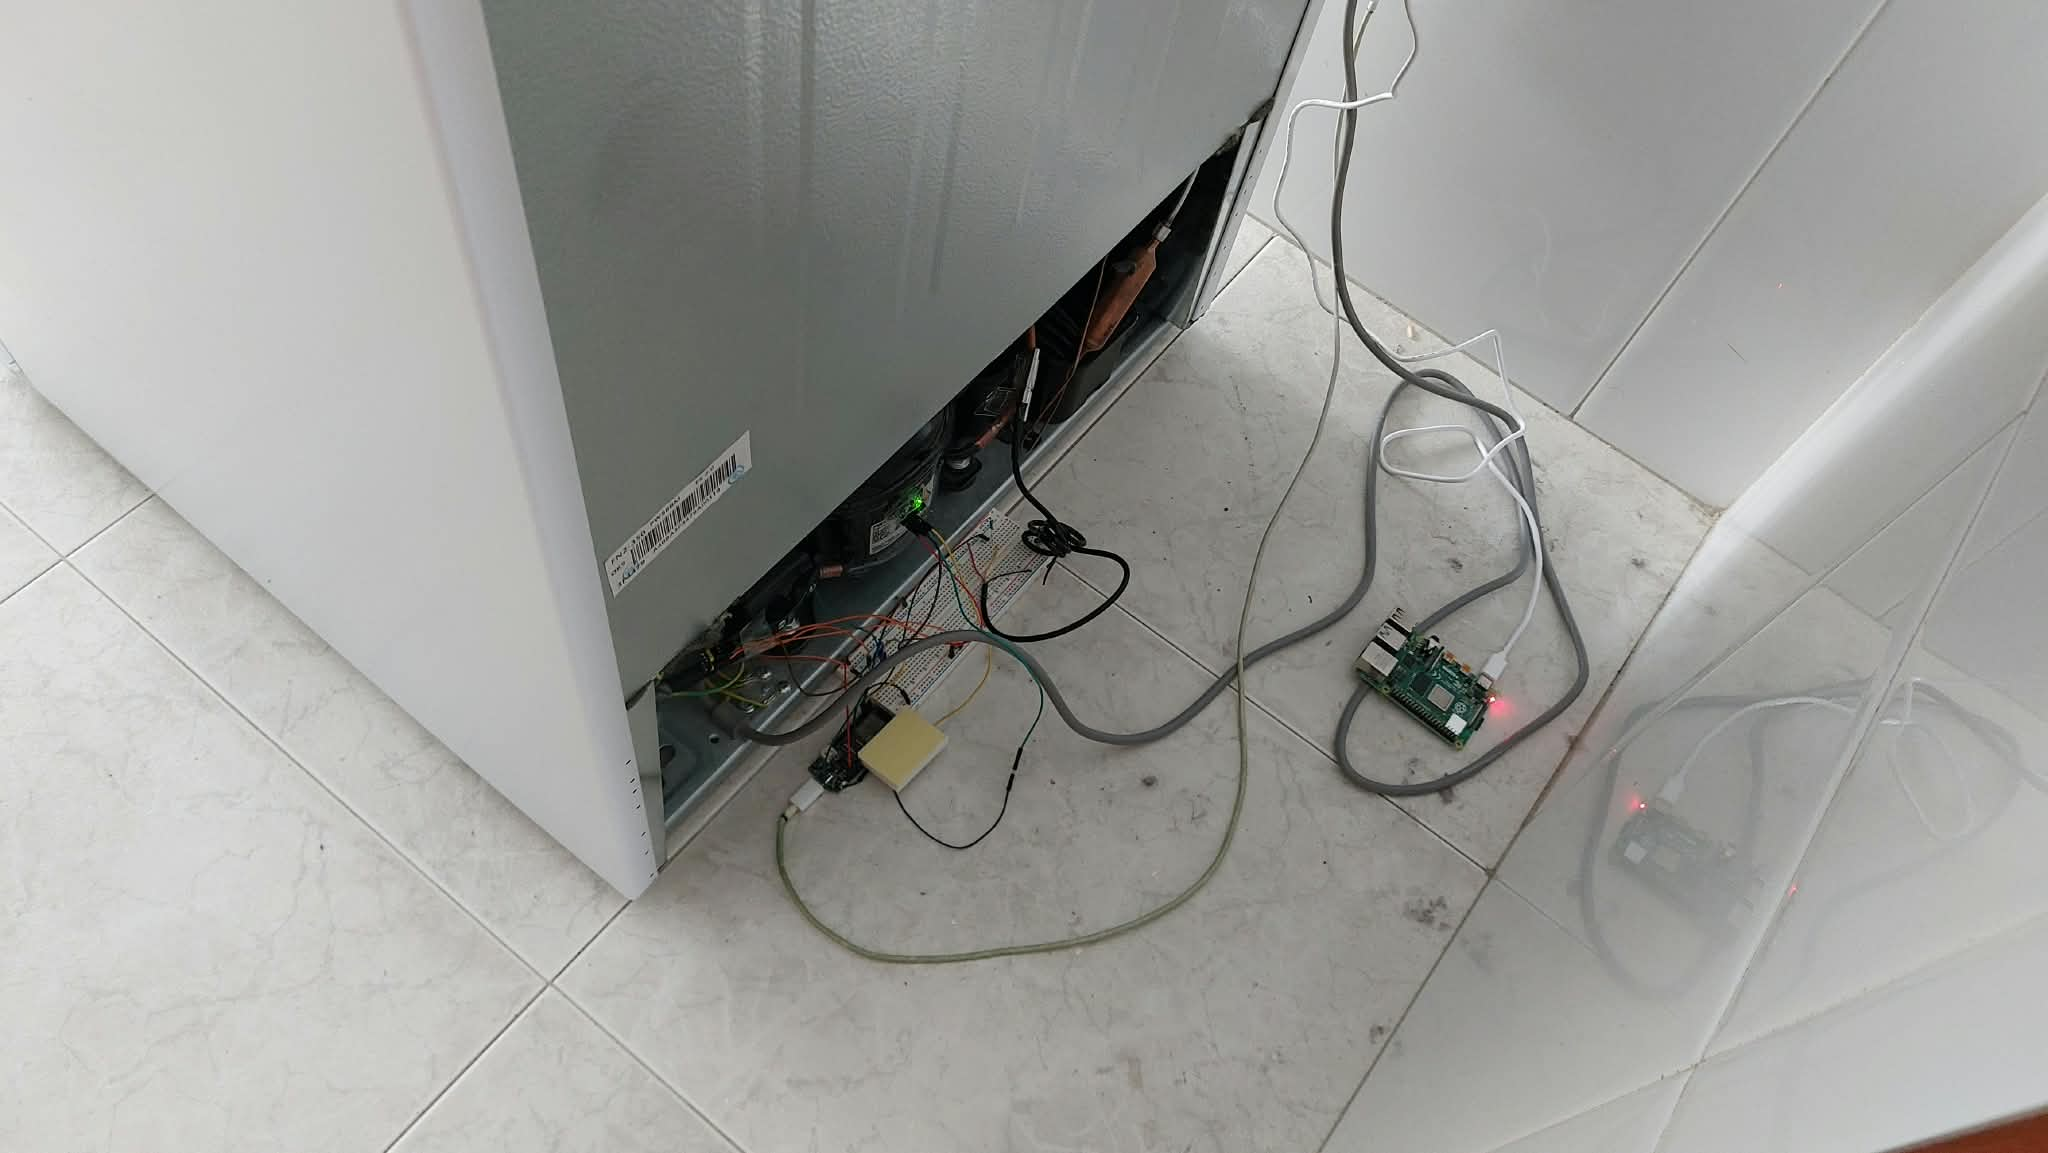
\includegraphics[width=0.92\textwidth]{figuras/banco-conjunto-hub.jpg}
\caption{Conjunto del banco de pruebas: activo de refrigeración, nodo de captura en su base
y concentrador Raspberry~Pi.}
\label{fig:banco-conjunto}
\end{figure}

La figura~\ref{fig:banco-fijacion} recoge el detalle de la fijación del acelerómetro sobre
el compresor del activo de referencia. El sensor se adhiere al lateral de la cúpula del
compresor hermético, y el cableado del bus discurre hasta la placa de prototipado situada en
la base del alojamiento.

\begin{figure}[ht!]
\centering
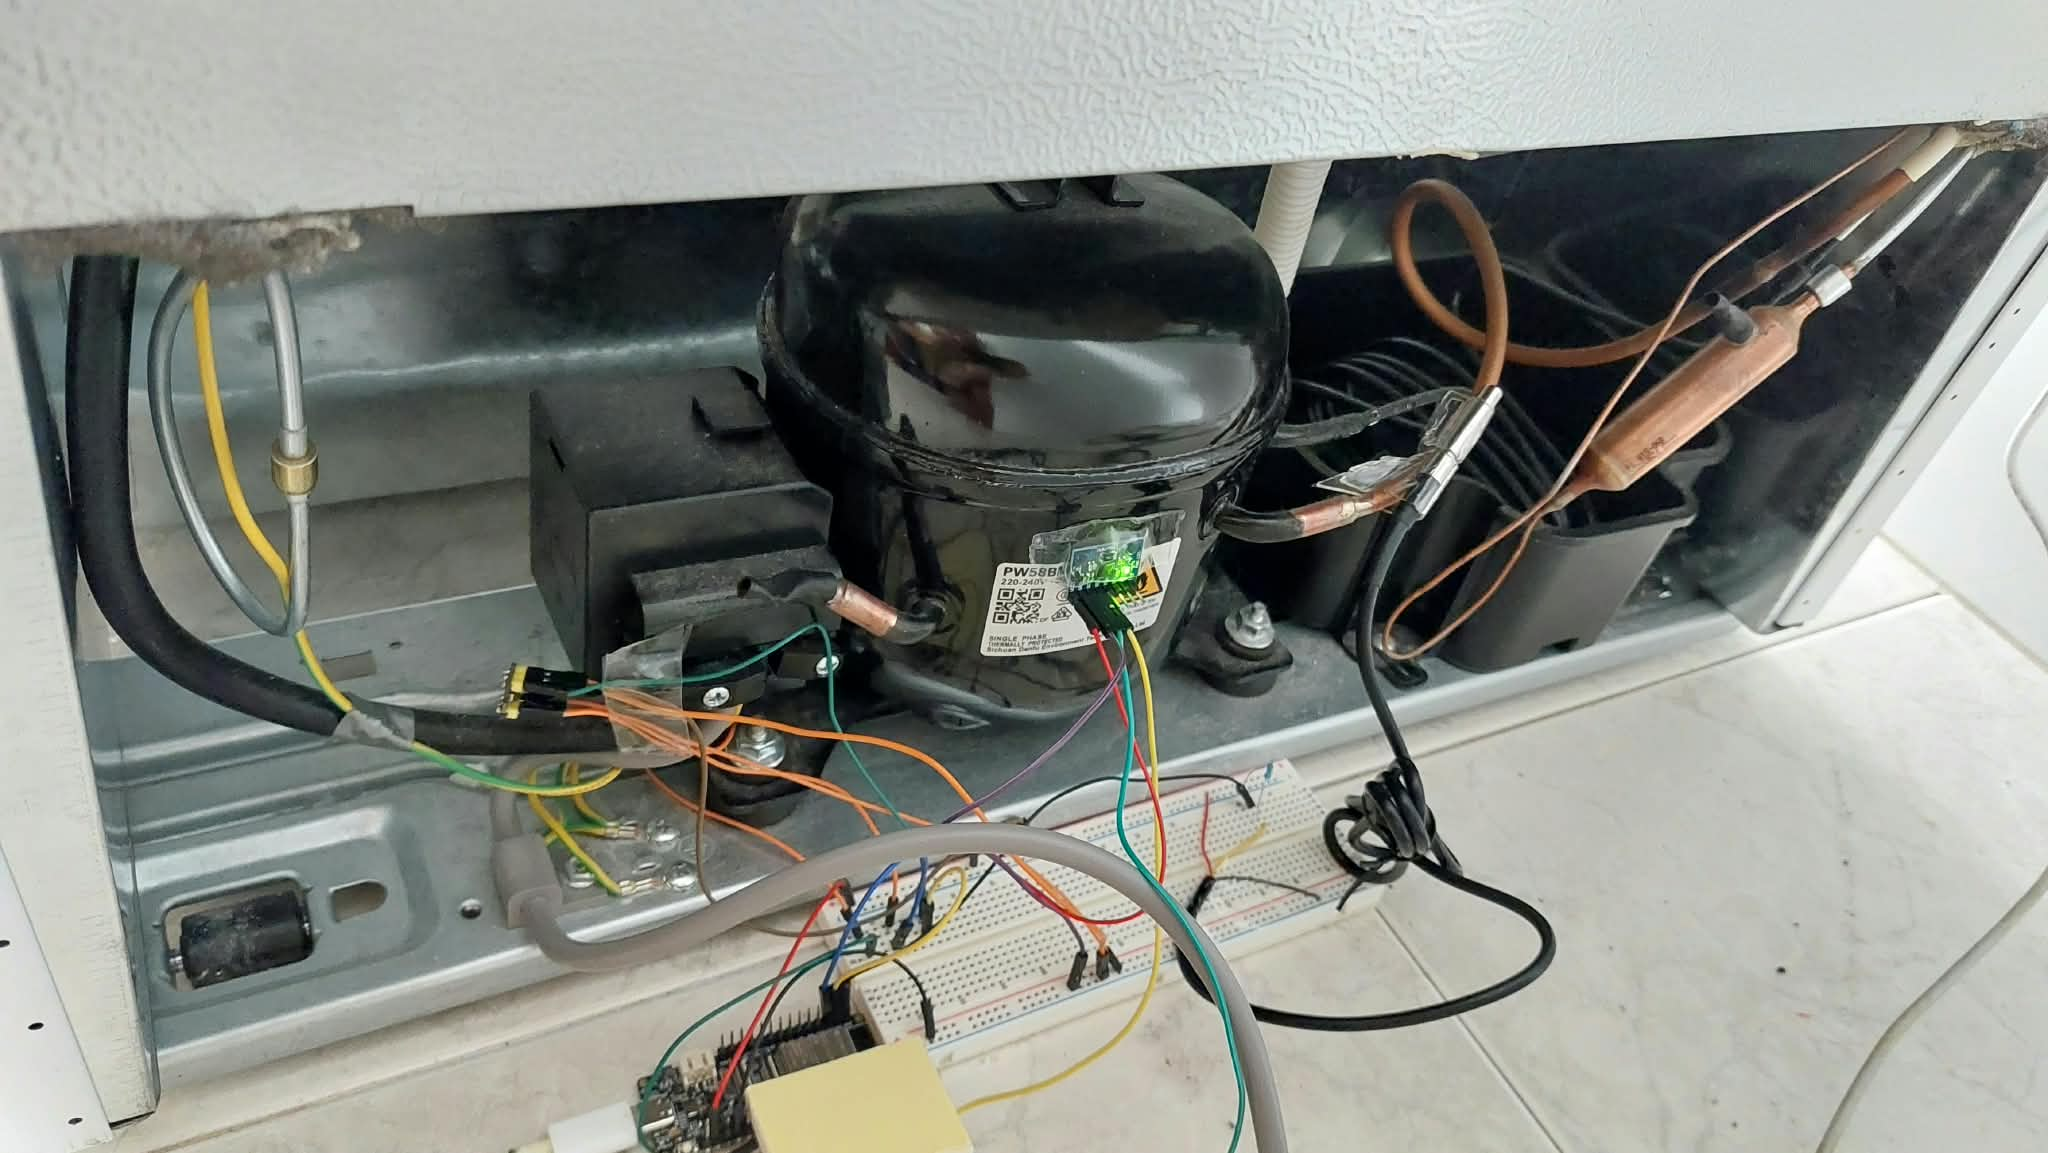
\includegraphics[width=0.92\textwidth]{figuras/banco-fijacion-sensor.jpg}
\caption{Detalle de la fijación del acelerómetro sobre la cúpula del compresor y del
cableado del bus I\textsuperscript{2}C hasta la placa de prototipado.}
\label{fig:banco-fijacion}
\end{figure}

\section{Selección del punto de medida}

La posición del acelerómetro resultó ser la decisión con mayor efecto sobre la calidad de la
medida, por encima del tipo de fijación. La figura~\ref{fig:puntos-medida} señala los tres
puntos evaluados sobre el compresor.

\begin{figure}[ht!]
\centering
\begin{tikzpicture}
  \node[inner sep=0] (foto)
    {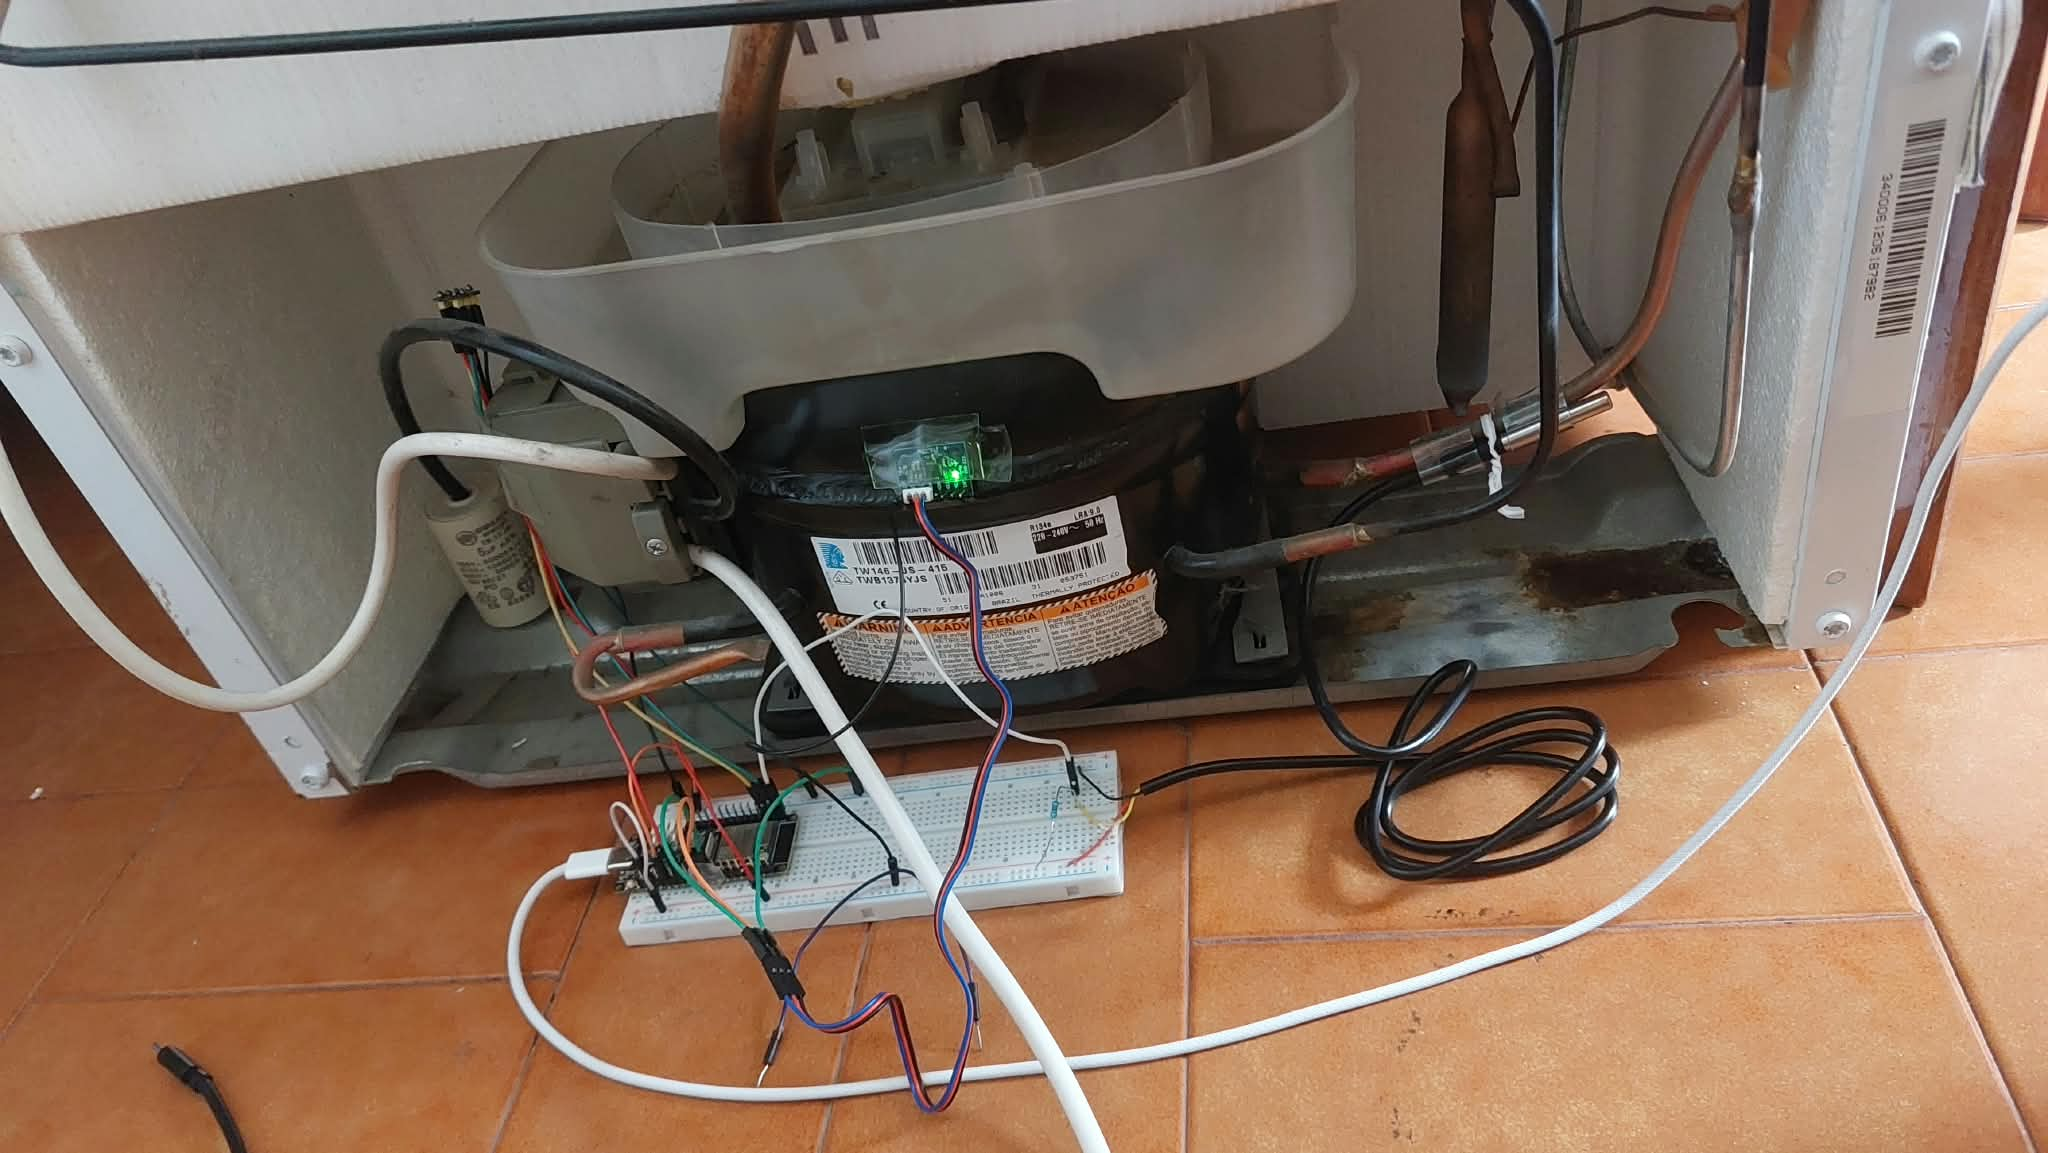
\includegraphics[width=0.94\textwidth]{figuras/banco-compresor-antiguo.jpg}};
  \begin{scope}[x={(foto.south east)}, y={(foto.north west)},
                marca/.style={circle, draw, line width=1.1pt, minimum size=15pt},
                etiq/.style={circle, fill, text=white, font=\bfseries\small,
                             inner sep=1.6pt, minimum size=13pt}]
    % Punto descartado: la cupula del compresor
    \draw[red!75!black, line width=1.1pt, dashed] (0.27,0.80) -- (0.44,0.63);
    \node[marca, red!75!black, minimum size=19pt] at (0.453,0.605) {};
    \node[red!75!black, font=\bfseries] at (0.453,0.605) {$\times$};
    \node[etiq, fill=red!75!black] at (0.255,0.815) {$\times$};

    % Punto 1: pata o anclaje al chasis
    \draw[orange!85!black, line width=1.1pt] (0.78,0.24) -- (0.63,0.40);
    \node[marca, orange!85!black] at (0.607,0.417) {};
    \node[etiq, fill=orange!85!black] at (0.795,0.225) {1};

    % Punto 2: tubo de descarga, el adoptado
    \draw[teal!80!black, line width=1.4pt] (0.17,0.24) -- (0.31,0.40);
    \node[marca, teal!80!black, line width=1.6pt, minimum size=17pt] at (0.326,0.421) {};
    \node[etiq, fill=teal!80!black] at (0.155,0.225) {2};
  \end{scope}
\end{tikzpicture}
\caption{Puntos de medida evaluados sobre el compresor. La cruz marca la cúpula, descartada;
el punto 1 el anclaje al chasis; el punto 2 el tubo de descarga, finalmente adoptado.}
\label{fig:puntos-medida}
\end{figure}

El cuadro~\ref{table:puntos-medida} recoge el resultado de la comparación.

\begin{table}[ht!]
\caption{Comparación de los puntos de medida evaluados.}
\label{table:puntos-medida}
\centering
\begin{tabular}{|p{3.4cm}|p{2.2cm}|p{2.4cm}|p{4.4cm}|}
\hline
\textbf{Punto} & \textbf{Valor eficaz} & \textbf{Fundamental} & \textbf{Resultado} \\
\hline
Cúpula del compresor & \mbox{0,047 m/s$^2$} & 4 de 52 ráfagas & Descartado \\
\hline
Tubo de descarga & \mbox{0,35--0,69 m/s$^2$} & 6 de 7 ráfagas & \textbf{Adoptado} \\
\hline
\end{tabular}
\end{table}

El motivo del descarte de la cúpula es de diseño del propio activo: un compresor hermético
lleva el conjunto motor-bomba suspendido sobre muelles \textit{dentro} de la carcasa, solución
que reduce el ruido transmitido y que, en consecuencia, aísla la superficie exterior de la
vibración que interesa medir. Midiendo en la cúpula se mide por el lado amortiguado de esa
suspensión.

El tubo de descarga, en cambio, está unido rígidamente al cuerpo de la bomba y transporta la
pulsación sin atravesar la suspensión interna. El cambio elevó el valor eficaz entre nueve y
veinte veces según el eje, y la frecuencia fundamental pasó de identificarse en el 8 \% de
las ráfagas a hacerlo en la práctica totalidad.

Procede precisar cómo se reparte esa mejora entre las características, porque el dato en
bruto induce a error. En torno al 95 \% del incremento reside en la componente tonal de alta
frecuencia analizada en el capítulo~\ref{cap:diseno}: el valor eficaz en la banda que
describen los estadísticos temporales es de \mbox{0,062 m/s$^2$} frente a los
\mbox{0,35 m/s$^2$} sin filtrar, de modo que la ganancia sobre esos estadísticos es de un
factor próximo a 1,6 y no de quince. La parte restante no es sin embargo señal desechable:
corresponde a la banda donde el capítulo~\ref{cap:resultados} identifica la firma del fallo.

La figura~\ref{fig:banco-antiguo} corresponde al montaje empleado durante la fase de
depuración del firmware, sobre un segundo activo de mayor antigüedad. Se incluye porque las
incidencias de integridad del bus descritas en el capítulo~\ref{cap:diseno} se
caracterizaron sobre este montaje.

\begin{figure}[ht!]
\centering
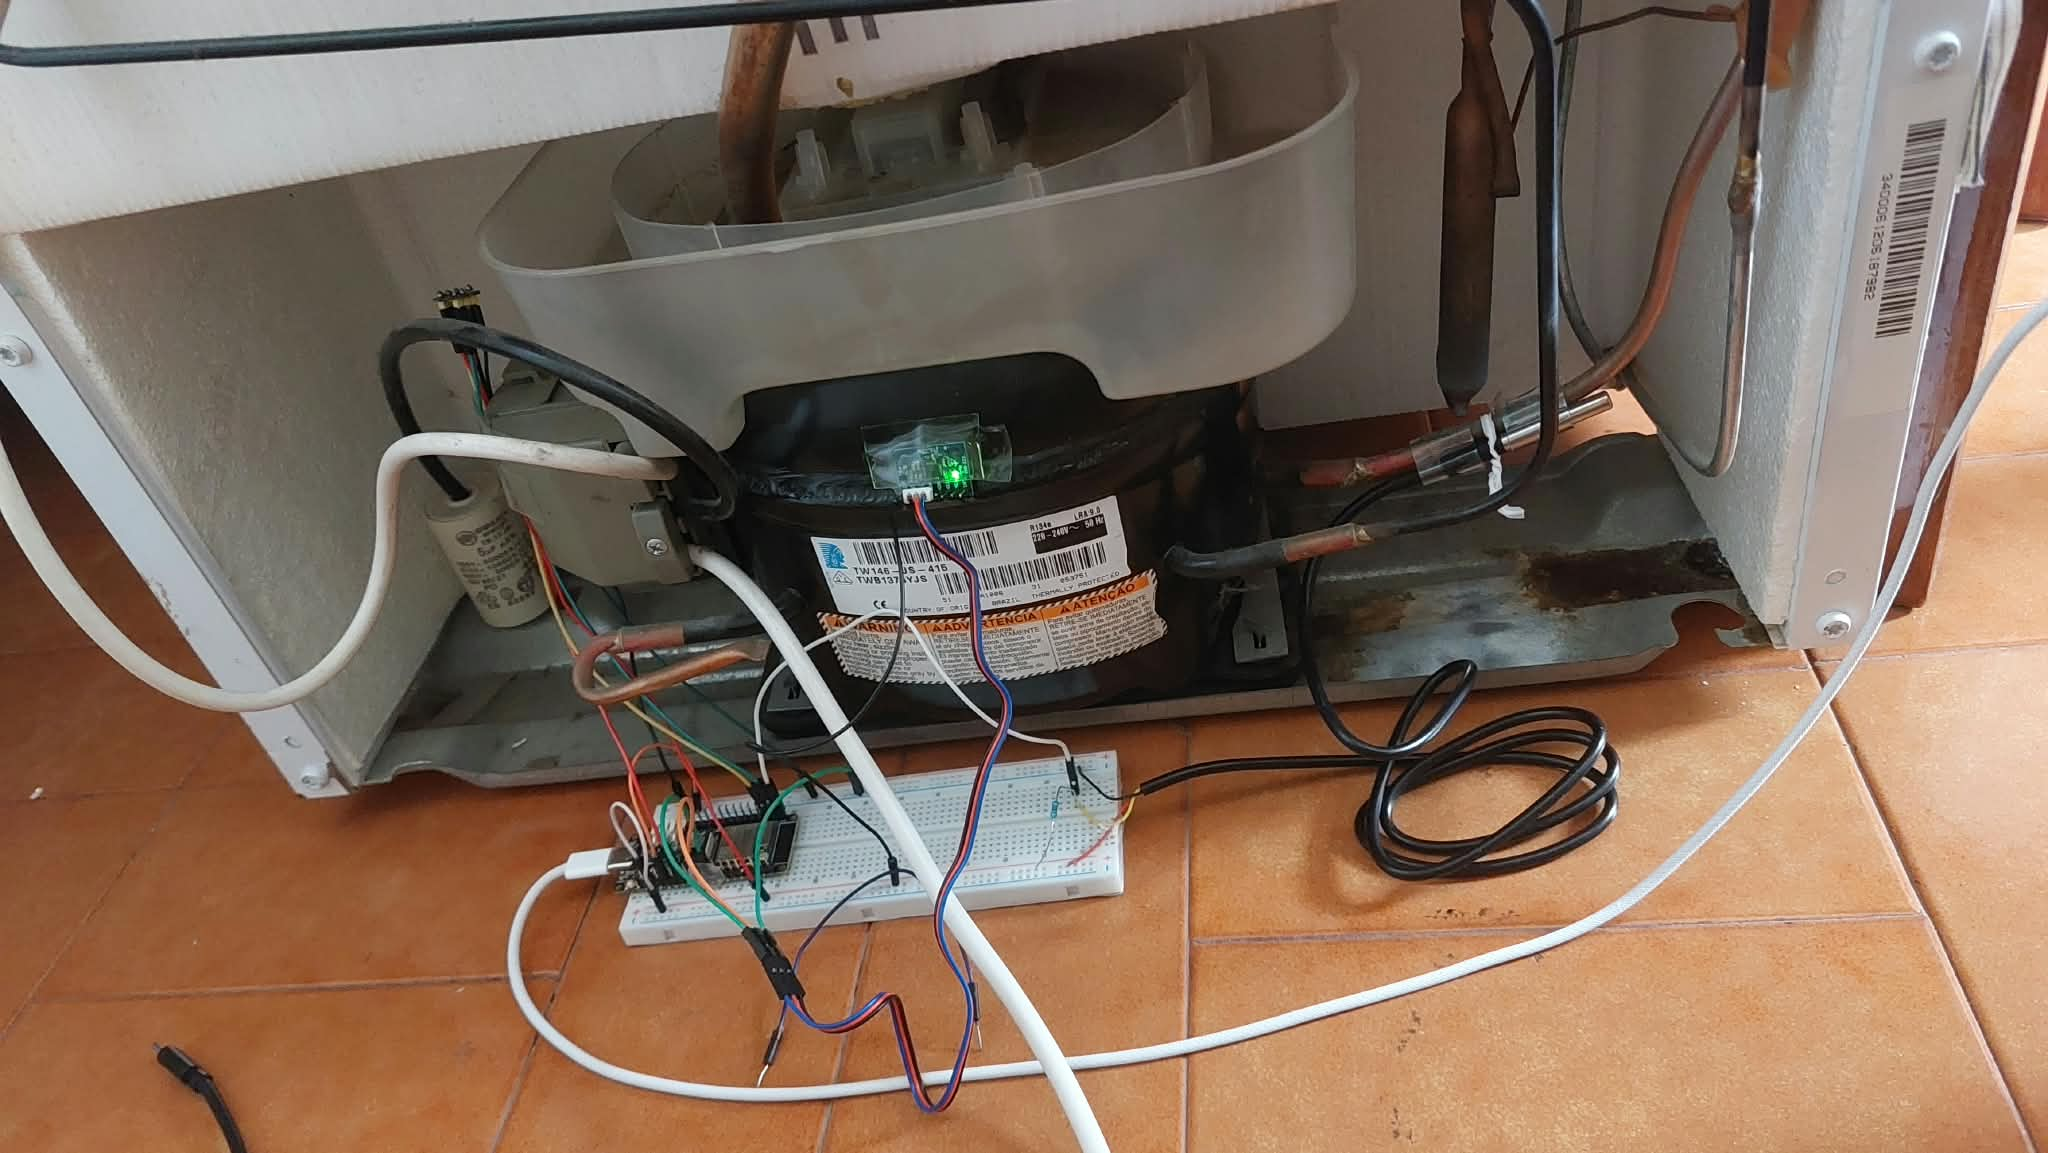
\includegraphics[width=0.92\textwidth]{figuras/banco-compresor-antiguo.jpg}
\caption{Montaje empleado en la fase de depuración, sobre un compresor de mayor antigüedad.}
\label{fig:banco-antiguo}
\end{figure}

\section{Limitaciones del montaje y su efecto sobre la medida}

Procede documentar de forma explícita las limitaciones del montaje, dado que condicionan la
calidad alcanzable del conjunto de datos y la interpretación de los resultados.

El acoplamiento del acelerómetro es adhesivo sobre una superficie curva, no una fijación
rígida atornillada. Una unión de este tipo se comporta como un acoplamiento elástico y
atenúa de forma selectiva el contenido de frecuencia más alta, que es precisamente el
informativo para el diagnóstico. La consecuencia esperable es una subestimación de la
amplitud de vibración y una reducción de la capacidad de discriminación del modelo.

El cableado del bus I\textsuperscript{2}C se realiza con conductores de prototipado sobre
placa de inserción, con una longitud del orden de \mbox{30 cm}, y discurre en paralelo al
cableado de alimentación del compresor, según se aprecia en la
figura~\ref{fig:banco-fijacion}. Este montaje presenta dos consecuencias medidas. La primera
es una tasa de fallo de lectura elevada, del orden de 37 reintentos por minuto con el activo
en marcha, atribuible a la pérdida intermitente de contacto en los conectores por efecto de
la vibración. La segunda es la posibilidad de acoplamiento de la frecuencia de red por
proximidad de conductores, circunstancia relevante porque el régimen de giro del compresor y
la frecuencia de red distan menos de dos veces la resolución espectral del análisis.

Estas limitaciones responden al alcance del trabajo, orientado a demostrar la viabilidad del
enfoque sobre una plataforma de prototipado, y no a producir un dispositivo de instalación
permanente. La decisión adoptada consiste en \textit{asumir} la tasa de fallo del cableado y
compensarla en el firmware mediante la validación de la transacción y el reintento acotado
descritos en el capítulo~\ref{cap:diseno}, en lugar de intervenir sobre el montaje físico. El
coste de esa decisión es una fracción de medidas descartadas mayor de la que tendría un
montaje soldado, cuantificada mediante los contadores de salud que el propio nodo publica.
Una implantación industrial exigiría conexiones soldadas con alivio de tensión y fijación
atornillada del sensor al chasis.

\section{Nota sobre los pines de configuración de arranque}

El pin GPIO~12 empleado para la señal de selección de canal del micrófono actúa como pin de
configuración de arranque en numerosas placas basadas en ESP32. Si la placa no arranca con
el micrófono conectado, procede reasignar esa señal a otra línea disponible.
